\section{Phương pháp nghiên cứu}
\label{sec:phuong-phap}

\subsection{Quy trình tổng quát và pipeline hai giai đoạn}

Báo cáo xây dựng một \textbf{pipeline hai giai đoạn} phát hiện DDoS, trong đó hai giai đoạn sử dụng hai bộ dữ liệu khác nhau với mục đích riêng biệt:

\begin{itemize}
    \item \textbf{Phase 1 -- Lựa chọn đặc trưng:} Áp dụng khung FAMS trên bộ dữ liệu tổng hợp từ Kaggle~\cite{kaggle_ddos_dataset} (CIC DoS 2016, CIC IDS 2017, CIC IDS 2018) để xác định tập đặc trưng gọn. Bộ dữ liệu Kaggle được lựa chọn ở bước này vì tính đa dạng về loại lưu lượng, phù hợp cho việc đánh giá tầm quan trọng đặc trưng trên nhiều điều kiện tấn công.
    \item \textbf{Phase 2 -- Huấn luyện và đánh giá:} Sử dụng tập đặc trưng từ Phase 1 để huấn luyện và đánh giá ba mô hình phân loại trên CIC-DDoS 2019~\cite{cicddos2019}. Bộ dữ liệu CIC-DDoS 2019 cung cấp đặc trưng flow-based chuẩn hóa và bao gồm nhiều nhóm tấn công riêng biệt, phù hợp cho thiết kế thực nghiệm tổng quát hóa.
\end{itemize}

Chi tiết từng bước của Phase 1 và Phase 2 được thể hiện trong Hình~\ref{fig:phase1_diagram} và Hình~\ref{fig:phase2_diagram}.

\begin{figure}[H]
\centering
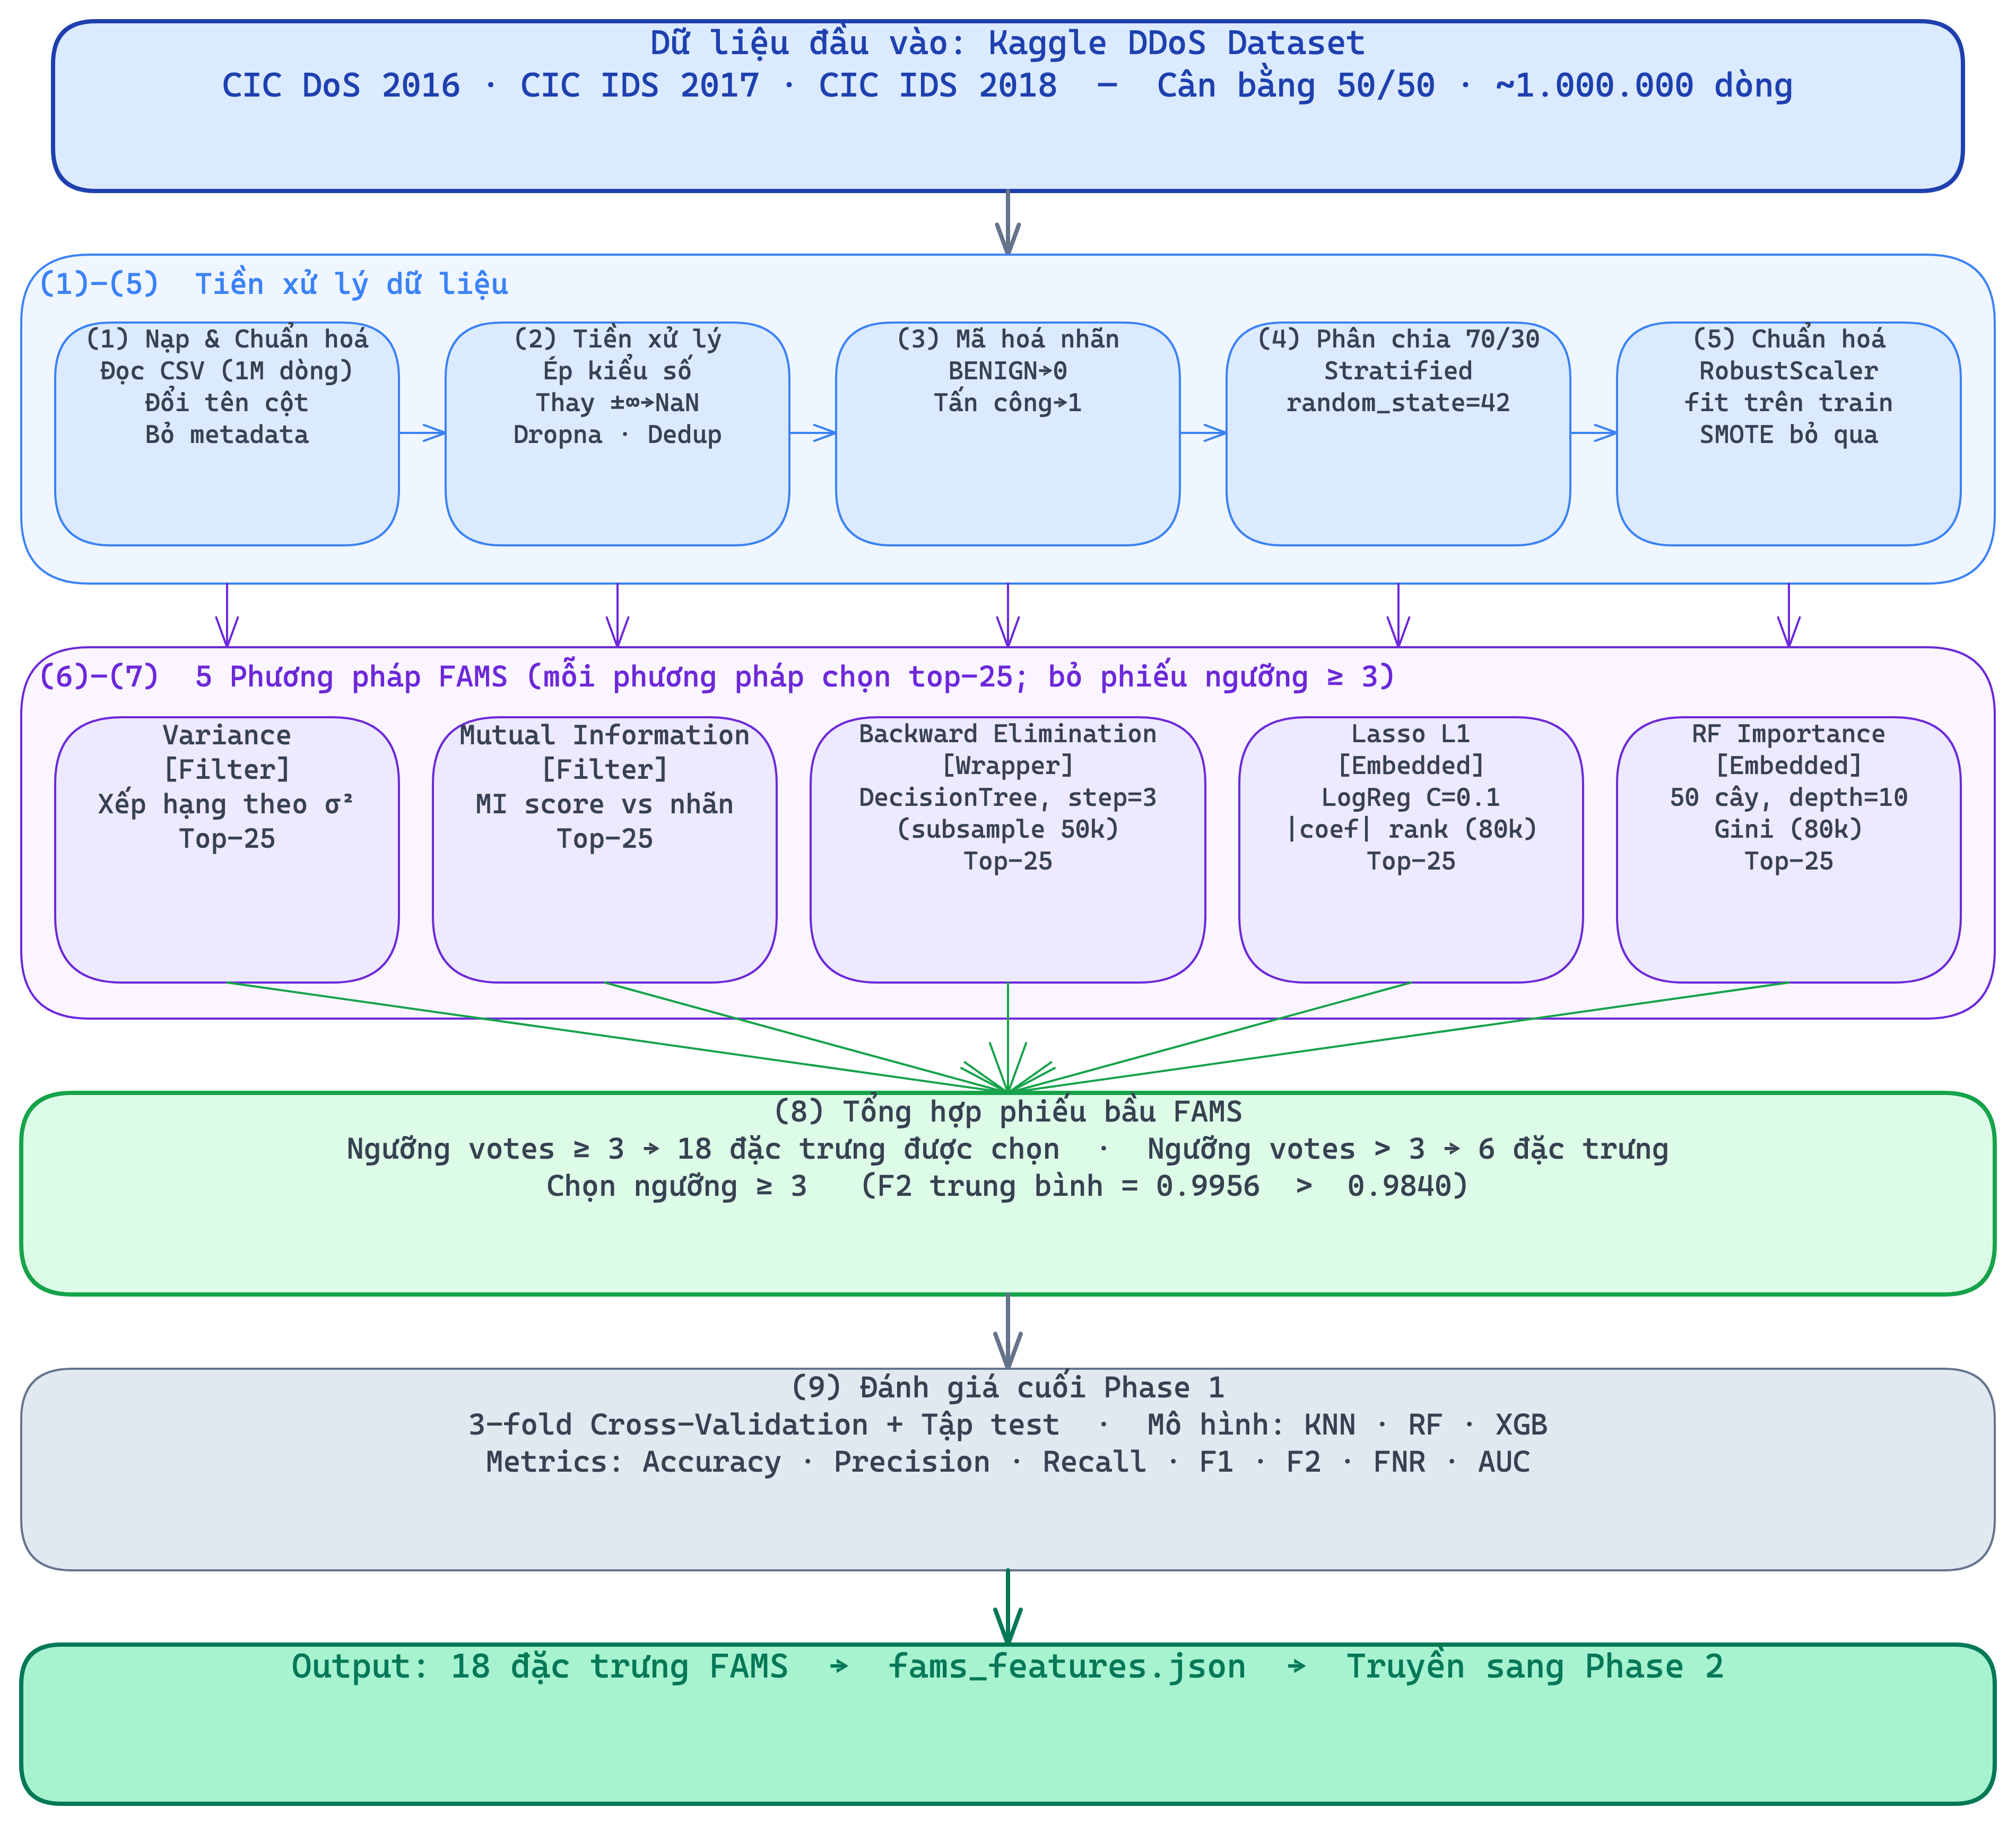
\includegraphics[width=\linewidth,keepaspectratio=true]{hinh/phase1_diagram_excalidraw.png}
\caption{Phase 1 -- Lựa chọn đặc trưng FAMS: từ dữ liệu Kaggle đến tập đặc trưng tối ưu.}
\label{fig:phase1_diagram}
\end{figure}

\begin{figure}[H]
\centering
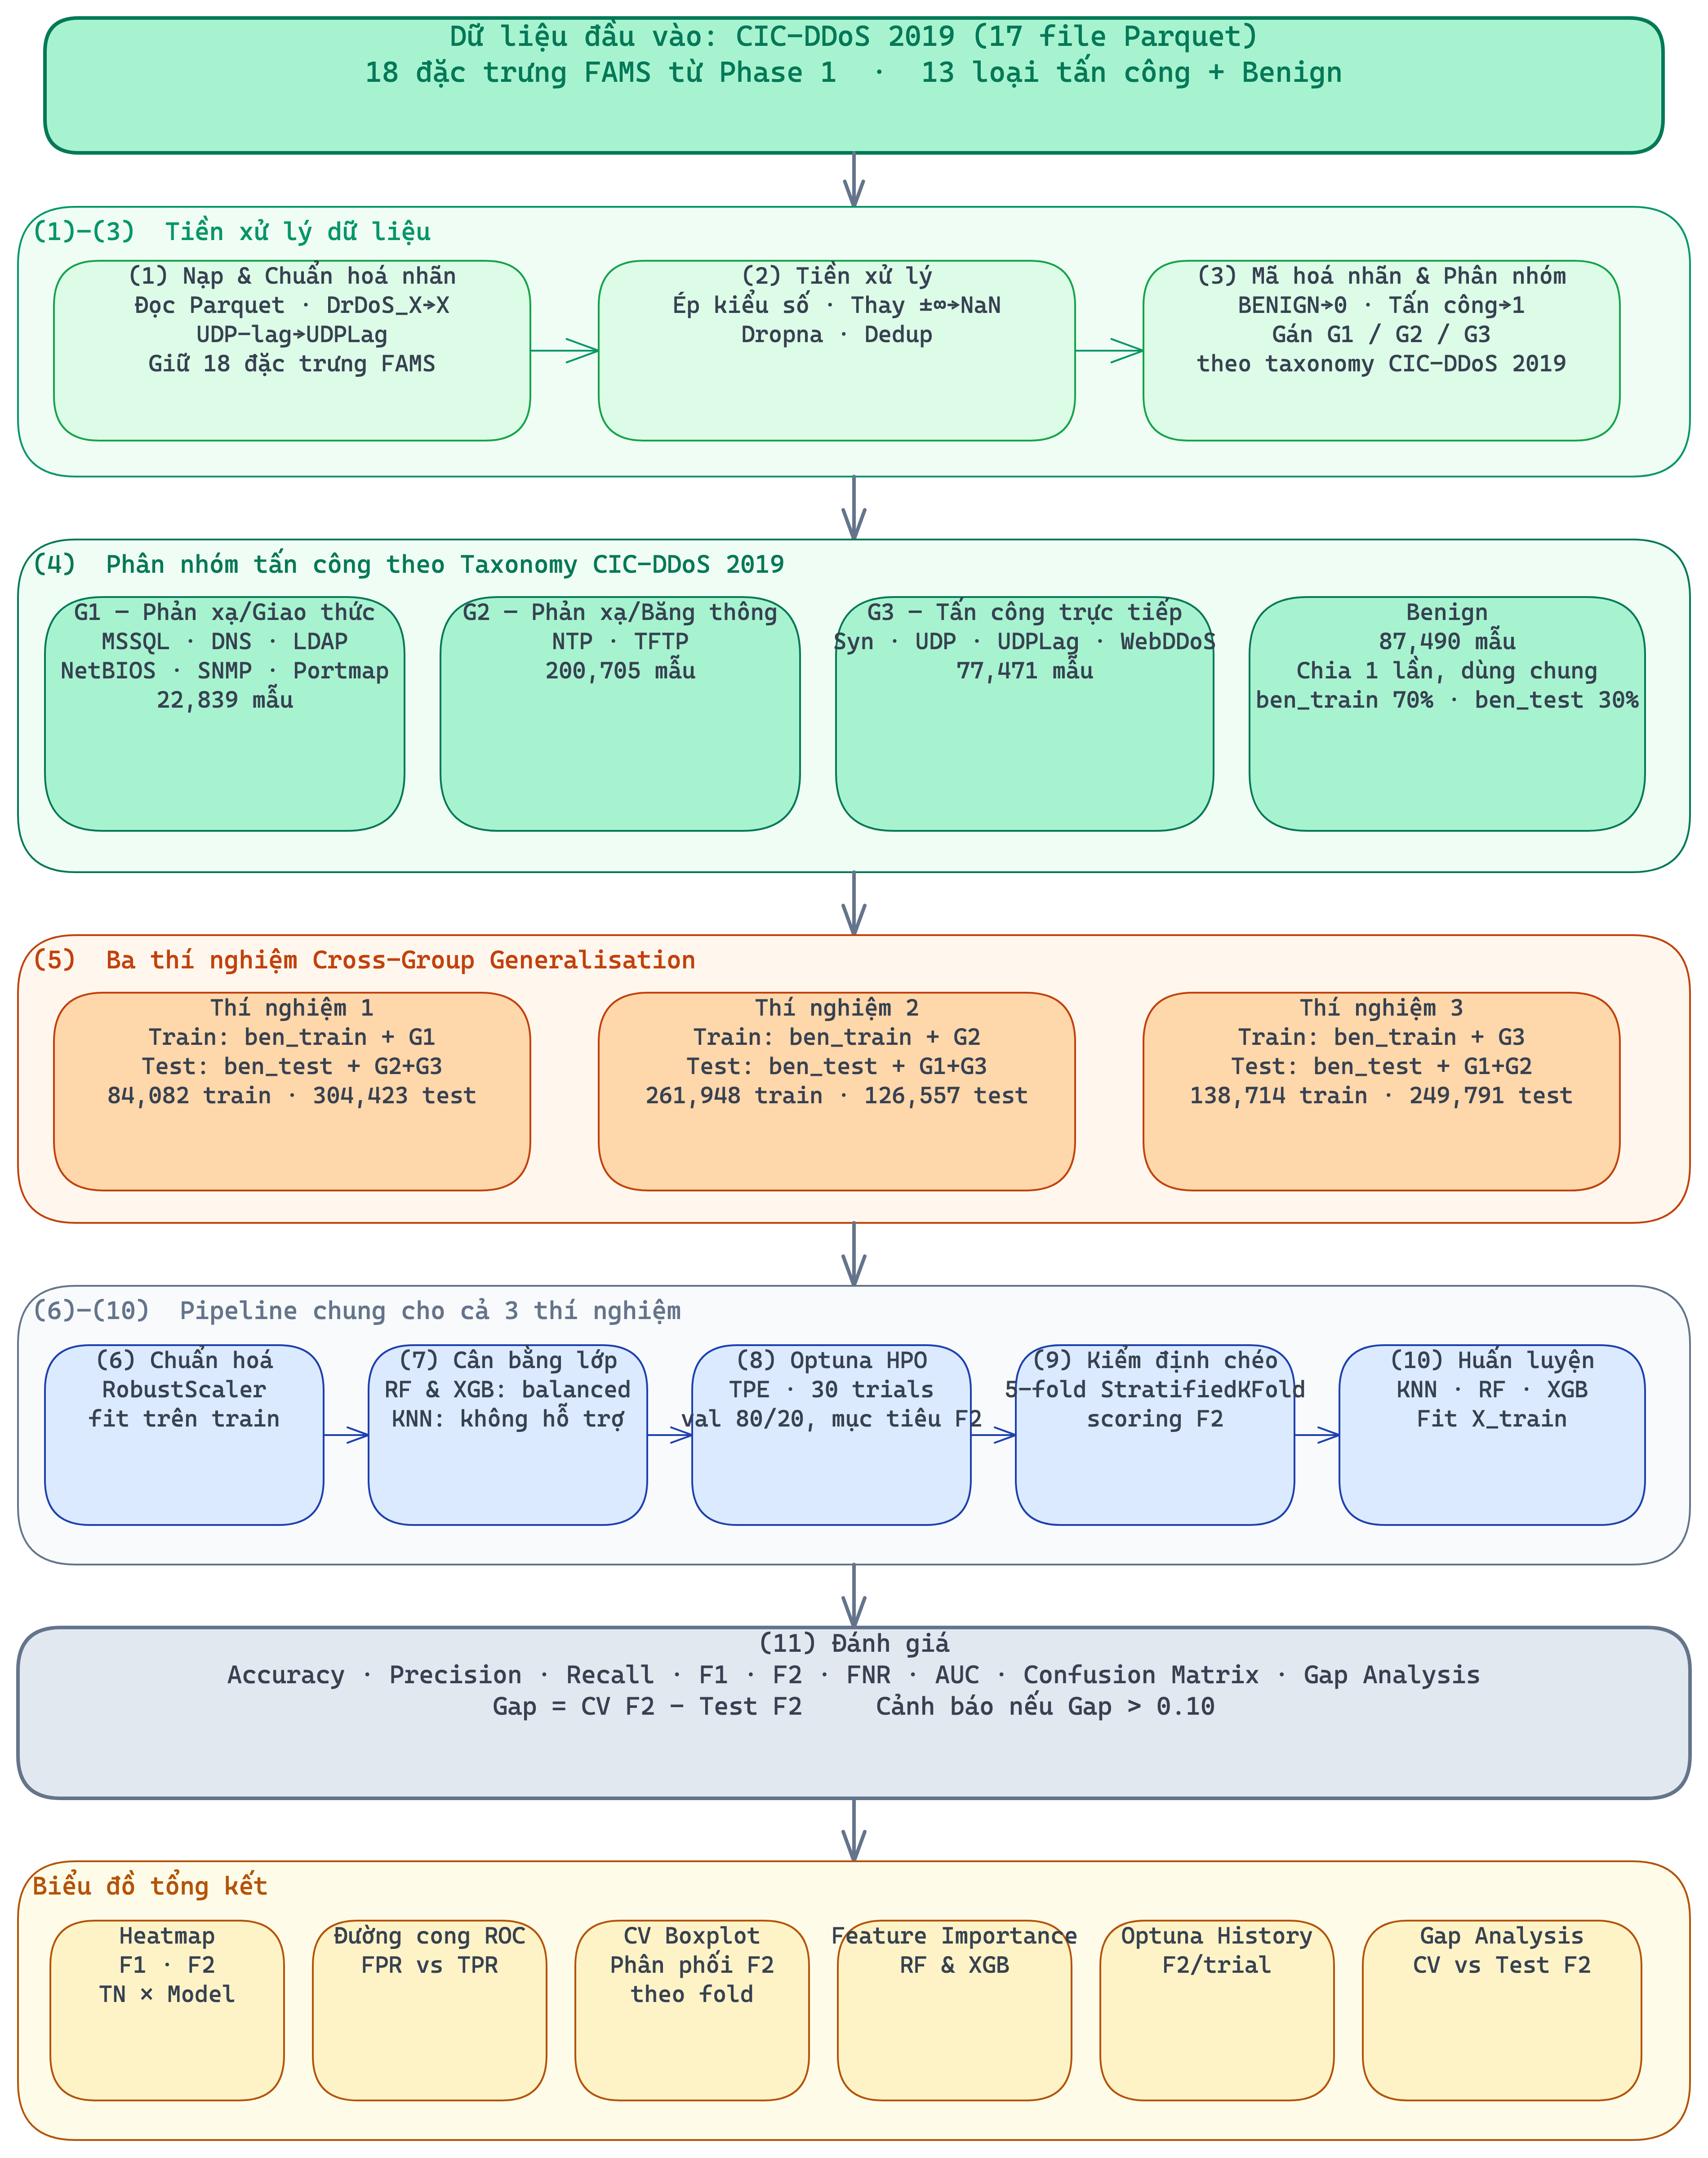
\includegraphics[width=\linewidth,keepaspectratio=true]{hinh/phase2_diagram_excalidraw.png}
\caption{Phase 2 -- Huấn luyện và đánh giá theo nhóm tấn công (Leave-One-Group-Out).}
\label{fig:phase2_diagram}
\end{figure}

\subsection{Dữ liệu và tiền xử lý}

\subsubsection{Bộ dữ liệu Phase 1 (Kaggle)}

Bộ dữ liệu tổng hợp từ Kaggle~\cite{kaggle_ddos_dataset} gộp lưu lượng từ ba bộ CIC DoS 2016, CIC IDS 2017 và CIC IDS 2018 thành một tập dữ liệu đã được cân bằng và chuẩn hóa nhãn. Đây là bộ dữ liệu flow-based với hơn 70 đặc trưng mô tả các thuộc tính thống kê của luồng mạng (kích thước gói tin, thời gian giữa các gói, số gói theo chiều forward/backward, v.v.). Sự đa dạng về loại lưu lượng của bộ này -- bao gồm nhiều kiểu DoS/DDoS cùng lưu lượng bình thường -- làm cho nó phù hợp cho bước lựa chọn đặc trưng.

\subsubsection{Bộ dữ liệu Phase 2 (CIC-DDoS 2019)}

CIC-DDoS 2019~\cite{cicddos2019} được tạo bởi Canadian Institute for Cybersecurity, cung cấp lưu lượng mạng flow-based ở định dạng Parquet gồm 17 file, tương ứng với nhiều loại tấn công DDoS hiện đại và lưu lượng bình thường (phân loại đầy đủ trong Hình~\ref{fig:cicddos2019_taxonomy}).

\begin{figure}[H]
\centering
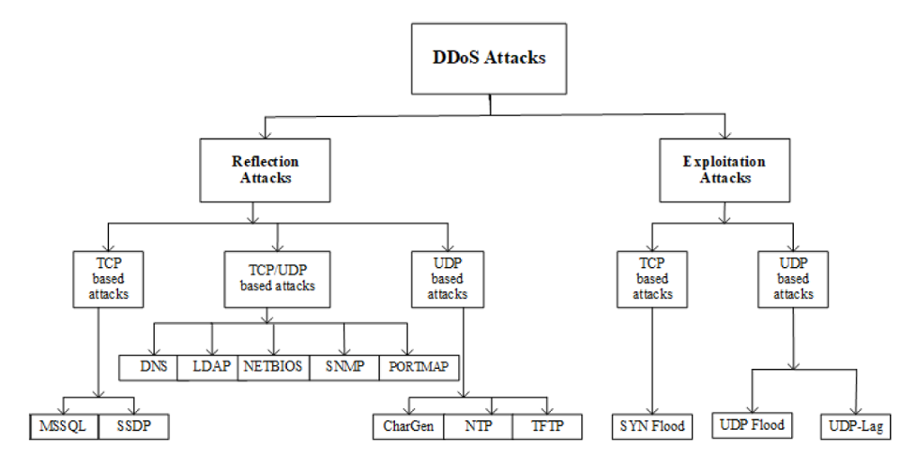
\includegraphics[width=\linewidth,keepaspectratio=true]{hinh/cicddos2019_taxonomy.png}
\caption{Phân loại tấn công DDoS trong bộ dữ liệu CIC-DDoS 2019~\cite{cicddos2019}.}
\label{fig:cicddos2019_taxonomy}
\end{figure} Sau tiền xử lý (loại bỏ hàng NaN, trùng lặp, và ép kiểu), bộ dữ liệu còn \textbf{388.505 dòng} (từ 431.371 dòng thô), bao gồm ba nhóm tấn công chính được sử dụng trong thiết kế thực nghiệm:
\begin{itemize}
    \item \textbf{G1 -- Reflection/Application:} MSSQL, DNS, LDAP, NetBIOS, SNMP, Portmap (22.839 mẫu tấn công).
    \item \textbf{G2 -- Reflection/Volume:} NTP, TFTP (200.705 mẫu).
    \item \textbf{G3 -- Exploitation:} Syn, UDP, UDPLag, WebDDoS (77.471 mẫu).
\end{itemize}
Lưu lượng Benign gồm \textbf{87.490 mẫu}, được chia ngẫu nhiên một lần theo tỷ lệ 70/30 (61.243 train / 26.247 test) và sử dụng chung cho cả ba thí nghiệm để đảm bảo tính nhất quán so sánh và tránh rò rỉ dữ liệu.

\subsubsection{Quy trình tiền xử lý chung}

Với cả hai bộ dữ liệu, quy trình tiền xử lý bao gồm:
\begin{enumerate}
    \item \textbf{Loại bỏ cột định danh:} Xóa các trường IP nguồn/đích, cổng, timestamp vì không mang thông tin tổng quát.
    \item \textbf{Xử lý giá trị thiếu và trùng lặp:} Loại bỏ hàng NaN và hàng trùng lặp hoàn toàn.
    \item \textbf{Chuẩn hóa nhãn:} Đưa nhãn về dạng thống nhất (ví dụ DrDoS\_DNS $\to$ DNS, UDP-lag $\to$ UDPLag).
    \item \textbf{Chuẩn hóa đặc trưng:} Áp dụng \textbf{RobustScaler}~\cite{pedregosa2011scikit} -- fit trên tập train, transform cả train và test -- để tránh data leakage và xử lý ngoại lai.
\end{enumerate}

\subsection{Thiết kế thực nghiệm: Leave-One-Group-Out}

Thiết kế thực nghiệm trung tâm của báo cáo là \textbf{Leave-One-Group-Out (LOGO)}: lần lượt sử dụng mỗi nhóm tấn công làm tập huấn luyện, trong khi các nhóm còn lại tạo thành tập kiểm thử. Cách tiếp cận này cho phép đánh giá trực tiếp \textit{khả năng tổng quát hóa liên nhóm} -- tức là mô hình học được từ một loại tấn công có phát hiện được các loại tấn công khác chưa từng thấy hay không.

Ba thí nghiệm được thiết kế như sau:
\begin{enumerate}
    \item \textbf{Exp 1:} Huấn luyện trên G1 + Benign (train) $\to$ Kiểm thử trên G2 + G3 + Benign (test).\\
    Kích thước: Train 84.082; Test 304.423.
    \item \textbf{Exp 2:} Huấn luyện trên G2 + Benign (train) $\to$ Kiểm thử trên G1 + G3 + Benign (test).\\
    Kích thước: Train 261.948; Test 126.557.
    \item \textbf{Exp 3:} Huấn luyện trên G3 + Benign (train) $\to$ Kiểm thử trên G1 + G2 + Benign (test).\\
    Kích thước: Train 138.714; Test 249.791.
\end{enumerate}

Trong mỗi thí nghiệm, tập Benign train được lấy từ phần 70\% đã chia cố định trước; tập Benign test là phần 30\% còn lại. Tập tấn công của nhóm huấn luyện được chia 70/30 theo stratified sampling~\cite{pedregosa2011scikit} để tạo tập train và tập validation nội bộ.

\subsection{Quy trình huấn luyện và tối ưu siêu tham số}

Với mỗi thí nghiệm và mỗi mô hình, quy trình huấn luyện gồm các bước:

\begin{enumerate}
    \item \textbf{Tối ưu siêu tham số bằng Optuna:} 30 trials với sampler TPE, mục tiêu tối đa hóa \textbf{F2-score} trung bình qua Stratified 5-Fold CV trên tập train. Tham số không gian tìm kiếm phụ thuộc mô hình (ví dụ: $k$ và metric khoảng cách cho KNN; số cây, độ sâu, số đặc trưng cho RF; learning rate, max depth, số rounds cho XGB).

    \item \textbf{Xử lý mất cân bằng lớp:} RF sử dụng \texttt{class\_weight='balanced'}; XGB dùng \texttt{scale\_pos\_weight} tỷ lệ nghịch với tần suất lớp; KNN không hỗ trợ cơ chế cân bằng lớp tường minh.

    \item \textbf{Huấn luyện mô hình cuối:} Sau khi tìm được siêu tham số tốt nhất, mô hình được huấn luyện lại trên \textit{toàn bộ} tập train (không chia fold).

    \item \textbf{Đánh giá trên tập test:} Mô hình được đánh giá trên tập test chứa các nhóm tấn công chưa thấy trong huấn luyện.
\end{enumerate}

\subsection{Chỉ số đánh giá}

Báo cáo sử dụng bộ chỉ số đánh giá sau, tính trên tập test hold-out:

\begin{itemize}
    \item \textbf{Accuracy:} Tỷ lệ dự đoán đúng tổng thể. Không phù hợp là chỉ số duy nhất do mất cân bằng lớp.
    \item \textbf{Precision:} $P = TP / (TP + FP)$. Trong số các mẫu được dự đoán là tấn công, bao nhiêu thực sự là tấn công.
    \item \textbf{Recall:} $R = TP / (TP + FN)$. Trong số các mẫu tấn công thực tế, bao nhiêu được phát hiện.
    \item \textbf{F1-Score:} Trung bình điều hòa của Precision và Recall ($\beta = 1$).
    \item \textbf{F2-Score:} Trung bình điều hòa có trọng số ($\beta = 2$), ưu tiên Recall. Đây là chỉ số chính của báo cáo.
    \item \textbf{FNR} (False Negative Rate): $FNR = FN / (FN + TP)$. Tỷ lệ tấn công bị bỏ sót; FNR càng thấp càng tốt.
    \item \textbf{AUC} (Area Under ROC Curve): Đánh giá khả năng phân biệt tổng thể của mô hình trên mọi ngưỡng quyết định.
    \item \textbf{Gap} $= \text{CV F2} - \text{Test F2}$: Chênh lệch giữa F2 nội bộ (cross-validation trên train) và F2 trên tập test. Gap dương lớn phản ánh mô hình overfit vào loại tấn công trong tập huấn luyện và tổng quát hóa kém.
    \item \textbf{Thời gian huấn luyện} (Training Time, giây): Thời gian huấn luyện mô hình cuối trên toàn bộ tập train sau khi đã tìm được siêu tham số tối ưu. Phản ánh chi phí tính toán offline của pipeline.
    \item \textbf{Thời gian suy luận} (Inference Time, ms/mẫu): Thời gian trung bình để mô hình phân loại một mẫu lưu lượng. Có ý nghĩa trực tiếp với yêu cầu phát hiện thời gian thực. Việc giảm số đặc trưng đầu vào từ 70+ xuống 18 (FAMS) kỳ vọng rút ngắn đáng kể chỉ số này, đặc biệt với KNN có chi phí suy luận tuyến tính theo số chiều.
\end{itemize}
